\element{mob}{
\begin{question}{mob 01}
Soit le schéma suivant. Donner la mobilité du mécanisme.
\begin{center}
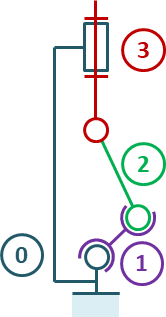
\includegraphics[width=3cm]{cas_01}
\end{center}
	\begin{reponses}	
	\bonne 2
	\mauvaise 0
	\mauvaise 1
	\mauvaise 3
	\end{reponses}
\end{question}\\}

\element{mob}{
\begin{question}{mob 02}
Soit le schéma suivant. Donner la mobilité du mécanisme.
\begin{center}
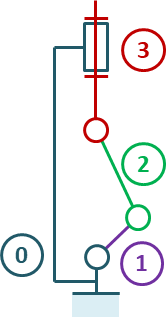
\includegraphics[width=3cm]{cas_02}
\end{center}
	\begin{reponses}	
	\bonne 0
	\mauvaise 1
	\mauvaise 2
	\mauvaise 3
	\end{reponses}
\end{question}\\}


\element{mob}{
\begin{question}{mob 03}
Soit le schéma suivant. Donner la mobilité du mécanisme.
\begin{center}
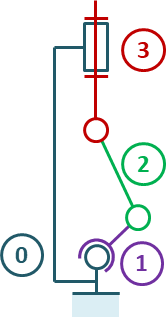
\includegraphics[width=3cm]{cas_03}
\end{center}
	\begin{reponses}	
	\bonne 1
	\mauvaise 0
	\mauvaise 2
	\mauvaise 3
	\end{reponses}
\end{question}\\}


\element{mob}{
\begin{question}{mob 04}
Soit le schéma suivant. Donner la mobilité du mécanisme.
\begin{center}
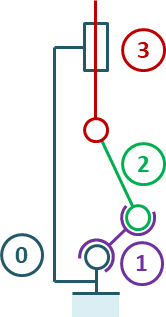
\includegraphics[width=3cm]{cas_04}
\end{center}
	\begin{reponses}	
	\bonne 3
	\mauvaise 0
	\mauvaise 1
	\mauvaise 2
	\end{reponses}
\end{question}\\}

\element{mob}{
\begin{question}{mob 05}
Soit le schéma suivant. Donner la mobilité du mécanisme.
\begin{center}
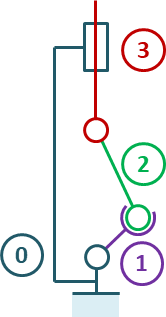
\includegraphics[width=3cm]{cas_05}
\end{center}
	\begin{reponses}	
	\bonne 1
	\mauvaise 0
	\mauvaise 2
	\mauvaise 3
	\end{reponses}
\end{question}\\}


\element{mob}{
\begin{question}{mob 06}
Soit le schéma suivant. Donner la mobilité du mécanisme.
\begin{center}
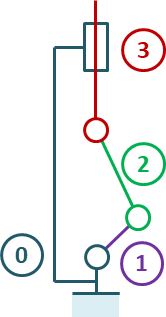
\includegraphics[width=3cm]{cas_06}
\end{center}
	\begin{reponses}	
	\bonne 1
	\mauvaise 0
	\mauvaise 2
	\mauvaise 3
	\end{reponses}
\end{question}\\}

\element{mob}{
\begin{question}{mob 07}
Soit le schéma suivant. Donner la mobilité du mécanisme.
\begin{center}
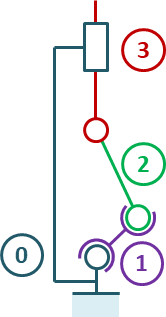
\includegraphics[width=3cm]{cas_07}
\end{center}
	\begin{reponses}	
	\bonne 2
	\mauvaise 0
	\mauvaise 1
	\mauvaise 3
	\end{reponses}
\end{question}\\}

\element{mob}{
\begin{question}{mob 08}
Soit le schéma suivant. Donner la mobilité du mécanisme.
\begin{center}
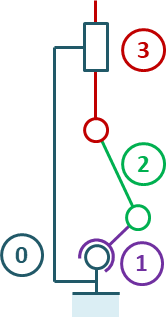
\includegraphics[width=3cm]{cas_08}
\end{center}
	\begin{reponses}	
	\bonne 1
	\mauvaise 0
	\mauvaise 2
	\mauvaise 3
	\end{reponses}
\end{question}\\}


\element{mob}{
\begin{question}{mob 09}
Soit le schéma suivant. Donner la mobilité du mécanisme.
\begin{center}
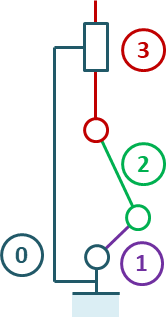
\includegraphics[width=3cm]{cas_09}
\end{center}
	\begin{reponses}	
	\bonne 3
	\mauvaise 0
	\mauvaise 1
	\mauvaise 2
	\end{reponses}
\end{question}\\}


\element{mob}{
\begin{question}{mob 10}
Soit le schéma suivant. Donner la mobilité du mécanisme.
\begin{center}
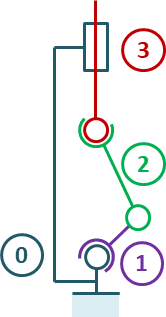
\includegraphics[width=3cm]{cas_10}
\end{center}
	\begin{reponses}	
	\bonne 3
	\mauvaise 0
	\mauvaise 1
	\mauvaise 2
	\end{reponses}
\end{question}\\}


\element{mob}{
\begin{question}{mob 11}
Soit le schéma suivant. Donner la mobilité du mécanisme.
\begin{center}
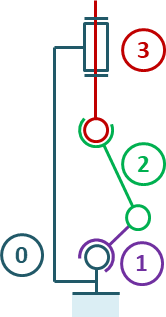
\includegraphics[width=3cm]{cas_11}
\end{center}
	\begin{reponses}	
	\bonne 2
	\mauvaise 0
	\mauvaise 1
	\mauvaise 3
	\end{reponses}
\end{question}\\}

\element{mob}{
\begin{question}{mob 12}
Soit le schéma suivant. Donner la mobilité du mécanisme.
\begin{center}
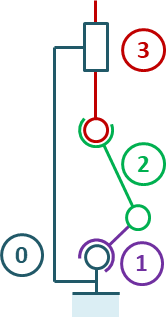
\includegraphics[width=3cm]{cas_12}
\end{center}
	\begin{reponses}	
	\bonne 2
	\mauvaise 0
	\mauvaise 1
	\mauvaise 3
	\end{reponses}
\end{question}\\}


\element{hs}{
\begin{question}{hs 01}
Soit le schéma suivant. Donner le degré d'hyperstatisme du mécanisme.
\begin{center}
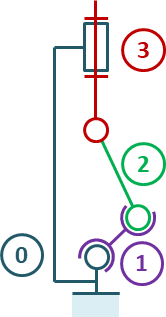
\includegraphics[width=3cm]{cas_01}
\end{center}
	\begin{reponses}	
	\bonne 0
	\mauvaise 1
	\mauvaise 2
	\mauvaise 3
	\end{reponses}
\end{question}\\}

\element{hs}{
\begin{question}{hs 02}
Soit le schéma suivant. Donner le degré d'hyperstatisme du mécanisme.
\begin{center}
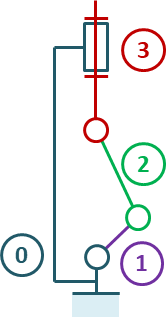
\includegraphics[width=3cm]{cas_02}
\end{center}
	\begin{reponses}	
	\bonne 2
	\mauvaise 0
	\mauvaise 1
	\mauvaise 3
	\end{reponses}
\end{question}\\}


\element{hs}{
\begin{question}{hs 03}
Soit le schéma suivant. Donner le degré d'hyperstatisme du mécanisme.
\begin{center}
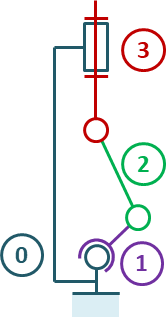
\includegraphics[width=3cm]{cas_03}
\end{center}
	\begin{reponses}	
	\bonne 1
	\mauvaise 0
	\mauvaise 2
	\mauvaise 3
	\end{reponses}
\end{question}\\}


\element{hs}{
\begin{question}{hs 04}
Soit le schéma suivant. Donner le degré d'hyperstatisme du mécanisme.
\begin{center}
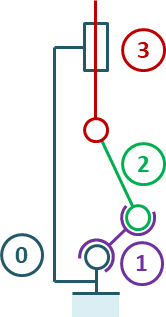
\includegraphics[width=3cm]{cas_04}
\end{center}
	\begin{reponses}	
	\bonne 0
	\mauvaise 3
	\mauvaise 1
	\mauvaise 2
	\end{reponses}
\end{question}\\}

\element{hs}{
\begin{question}{hs 05}
Soit le schéma suivant. Donner le degré d'hyperstatisme du mécanisme.
\begin{center}
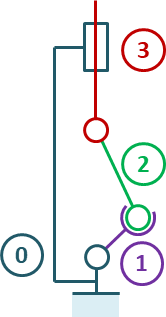
\includegraphics[width=3cm]{cas_05}
\end{center}
	\begin{reponses}	
	\bonne 0
	\mauvaise 1
	\mauvaise 2
	\mauvaise 3
	\end{reponses}
\end{question}\\}


\element{hs}{
\begin{question}{hs 06}
Soit le schéma suivant. Donner le degré d'hyperstatisme du mécanisme.
\begin{center}
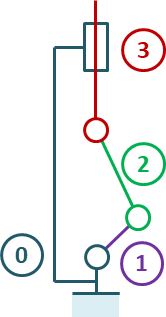
\includegraphics[width=3cm]{cas_06}
\end{center}
	\begin{reponses}	
	\bonne 2
	\mauvaise 0
	\mauvaise 1
	\mauvaise 3
	\end{reponses}
\end{question}\\}

\element{hs}{
\begin{question}{hs 07}
Soit le schéma suivant. Donner le degré d'hyperstatisme du mécanisme.
\begin{center}
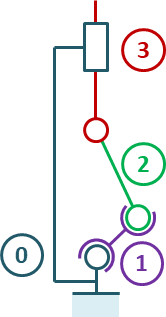
\includegraphics[width=3cm]{cas_07}
\end{center}
	\begin{reponses}	
	\bonne 0
	\mauvaise 1
	\mauvaise 2
	\mauvaise 3
	\end{reponses}
\end{question}\\}

\element{hs}{
\begin{question}{hs 08}
Soit le schéma suivant. Donner le degré d'hyperstatisme du mécanisme.
\begin{center}
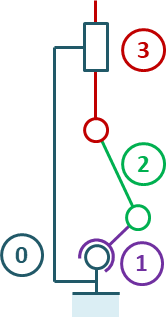
\includegraphics[width=3cm]{cas_08}
\end{center}
	\begin{reponses}	
	\bonne 1
	\mauvaise 0
	\mauvaise 2
	\mauvaise 3
	\end{reponses}
\end{question}\\}


\element{hs}{
\begin{question}{hs 09}
Soit le schéma suivant. Donner le degré d'hyperstatisme du mécanisme.
\begin{center}
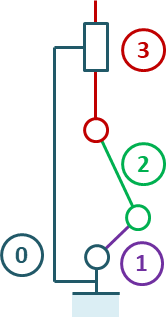
\includegraphics[width=3cm]{cas_09}
\end{center}
	\begin{reponses}	
	\bonne 3
	\mauvaise 0
	\mauvaise 2
	\mauvaise 1
	\end{reponses}
\end{question}\\}


\element{hs}{
\begin{question}{hs 10}
Soit le schéma suivant. Donner le degré d'hyperstatisme du mécanisme.
\begin{center}
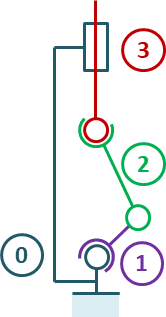
\includegraphics[width=3cm]{cas_10}
\end{center}
	\begin{reponses}	
	\bonne 0
	\mauvaise 1
	\mauvaise 2
	\mauvaise 3
	\end{reponses}
\end{question}\\}


\element{hs}{
\begin{question}{hs 11}
Soit le schéma suivant. Donner le degré d'hyperstatisme du mécanisme.
\begin{center}
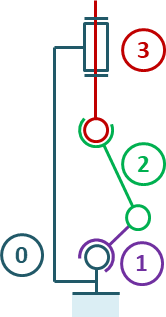
\includegraphics[width=3cm]{cas_11}
\end{center}
	\begin{reponses}	
	\bonne 0
	\mauvaise 1
	\mauvaise 2
	\mauvaise 3
	\end{reponses}
\end{question}\\}

\element{hs}{
\begin{question}{hs 12}
Soit le schéma suivant. Donner le degré d'hyperstatisme du mécanisme.
\begin{center}
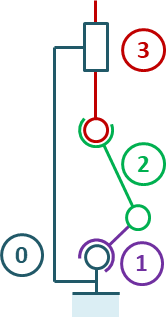
\includegraphics[width=3cm]{cas_12}
\end{center}
	\begin{reponses}	
	\bonne 0
	\mauvaise 1
	\mauvaise 2
	\mauvaise 3
	\end{reponses}
\end{question}\\}


